\documentclass[10pt,review,sigplan,anonymous=true]{acmart}
\settopmatter{printfolios=false,printccs=false,printacmref=false}

\bibliographystyle{ACM-Reference-Format}
\citestyle{acmauthoryear}   %% For author/year citations
\usepackage{listings,multirow,wrapfig,xspace,paralist}
\usepackage{xcolor,tikz,graphicx, pifont}
%\usetikzlibrary{positioning}

%% \newcommand{\authorcomment}[3]{\xspace\textcolor{#1}{{\bf #2} #3}\xspace}
\newcommand{\authorcomment}[3]{}
% For author notes:
\newcommand{\AG}[1]{\authorcomment{orange}{AG}{#1}}
\newcommand{\JV}[1]{\authorcomment{red}{JV}{#1}}

% For meta comments:
\newcommand{\isit}[1]{\authorcomment{cyan}{Check}{#1}}
\newcommand{\todo}[1]{\authorcomment{red}{TODO}{#1}}
\newcommand{\xmark}{\textcolor{red}{\ding{55}}}
\newcommand{\cmark}{\textcolor{green}{\ding{51}}}

\definecolor{LightGray}{RGB}{247, 247, 247}
\definecolor{Gray}{rgb}{.3,.3,.3}
\definecolor{DarkGray}{rgb}{.5,.5,.5}

%% https://www.davehofmann.de/defining-custom-language-templates-for-latex-listings/
% Define Language
\lstdefinelanguage{smalleR} {
  % list of keywords
  morekeywords={
    for,
    if,
    else,
    function
  },
  sensitive=true, % keywords are not case-sensitive
  morecomment=[l]{\#}, % l is for line comment
  morestring=[b]{"} % defines that strings are enclosed in double quotes
}

\lstset{
  language={smalleR},
  columns=flexible,
  captionpos=b,
  frame=single,
  framerule=0pt,
  framexleftmargin=1mm,
  framexrightmargin=1mm,
  tabsize=2,
  belowskip=0pt,
  basicstyle=\small\ttfamily,
  backgroundcolor=\color{LightGray},
  emphstyle=\sffamily,
  keywordstyle=\bfseries,
  commentstyle=\color{Gray}\em,
  stringstyle=\color{Gray},
  alsoletter={., _, $},
  breaklines=true
}

\newcommand{\code}[1]{\lstinline |#1|\xspace}
\renewcommand{\c}[1]{\lstinline |#1|\xspace}
\newcommand{\eg}{\emph{e.g.},\xspace}
\newcommand{\ie}{\emph{i.e.},\xspace}

\newcommand{\environmentFun}{\code{environment}}
\newcommand{\asEnvironment}{\code{as.environment}}

\newcommand{\emptyenv}{\code{empyenv}}
\newcommand{\globalenv}{\code{globalenv}}

\newcommand{\base}{\code{base}}
\newcommand{\methods}{\code{methods}}
\newcommand{\lazyLoadDBexec}{\code{lazyLoadDBexec}}

\newcommand{\newEnv}{\code{new.env}}

\newcommand{\asList}{\code{as.list}}
\newcommand{\listToEnv}{\code{list2env}}

\newcommand{\ls}{\code{ls}}
\newcommand{\objects}{\code{objects}}

\newcommand{\subDollar}{\code{$}}
\newcommand{\subBracket}{\code{[[}}

\newcommand{\exist}{\code{exist}}

\newcommand{\get}{\code{get}}
\newcommand{\getZero}{\code{get0}}
\newcommand{\mget}{\code{mget}}
\newcommand{\dynGet}{\code{dynGet}}

\newcommand{\assign}{\code{assign}}

\newcommand{\remove}{\code{remove}}
\renewcommand{\rm}{\code{rm}}

\newcommand{\lockEnvironment}{\code{lockEnvironment}}
\newcommand{\lockBinding}{\code{lockBinding}}
\newcommand{\unlockBinding}{\code{unlockBinding}}

\newcommand{\eval}{\code{eval}}
\newcommand{\substitute}{\code{substitute}}

\newcommand{\parentEnv}{\code{parent.env}}
\newcommand{\parentEnvAssign}{\code{parent.env<-}}

\newcommand{\envtracer}{{\sf envtracer}\xspace}
\newcommand{\experimentr}{{\sf experimentr}\xspace}
\newcommand{\rdyntrace}{{\sf R-dyntrace}\xspace}

\newcommand{\ggplot}{\textit{ggplot2}\xspace}
\newcommand{\vctrs}{\textit{vctrs}\xspace}

%%% \setcopyright{rightsretained}
%%% \acmPrice{}
%%% \acmDOI{10.1145/3360579}
%%% \acmYear{2019}
%%% \copyrightyear{2019}
%%% \acmJournal{PACMPL}
%%% \acmVolume{3}
%%% \acmNumber{OOPSLA}
%% \acmArticle{153}
%%% \acmMonth{10}
\begin{document}
\title{On the Use of First-Class Environments in R}

\author{Aviral Goel}\affiliation{\institution{Northeastern University}\country{USA}}
\author{Jan Vitek}\affiliation{\institution{Czech Technical University and Northeastern University}\country{USA}}
\authorsaddresses{}
\renewcommand{\shortauthors}{Goel, et al.}


\begin{abstract}
  The R programming language is widely used for statistical computations. R
  encourages a very dynamic programming style, to enable interactive data
  exploration and rapid prototyping. A key enabler of this dynamism is its
  support for first-class environments. To our knowledge, R is the only
  mainstream programming language with explicit environments. This paper
  presents the design of environments in R, and an empirical evaluation of how
  they are used. For this, we analyze \AG{XXXX} programs from 100 most popular CRAN
  packages. We find that first-class environments are used for \AG{XYZ}.
\end{abstract}

\begin{CCSXML}
<ccs2012>
<concept>
<concept_id>10002944.10011123.10010912</concept_id>
<concept_desc>General and reference~Empirical studies</concept_desc>
<concept_significance>500</concept_significance>
</concept>
<concept>
<concept_id>10011007.10011006.10011008</concept_id>
<concept_desc>Software and its engineering~General programming languages</concept_desc>
<concept_significance>500</concept_significance>
</concept>
<concept>
<concept_id>10011007.10011006.10011050.10010517</concept_id>
<concept_desc>Software and its engineering~Scripting languages</concept_desc>
<concept_significance>500</concept_significance>
</concept>
<concept>
<concept_id>10011007.10011006.10011039.10011311</concept_id>
<concept_desc>Software and its engineering~Semantics</concept_desc>
<concept_significance>300</concept_significance>
</concept>
</ccs2012>
\end{CCSXML}

\ccsdesc[500]{General and reference~Empirical studies}
\ccsdesc[500]{Software and its engineering~General programming languages}
\ccsdesc[500]{Software and its engineering~Scripting languages}
\ccsdesc[300]{Software and its engineering~Semantics}

%\keywords{R language, delayed or lazy evaluation}

\maketitle
\section{Introduction}

{\small \medskip\noindent\emph{Availability.} Our work is in open source, experiments are
repeatable and will be submitted to the AEC.}

\section{Background}\label{sec:background}

\subsection{Related Work}

There are three strands of related work: research on the R language, research on
supporting first-class environments, and first-class environments in contemporary
languages.

\paragraph{The R language} \citet{ecoop12} evaluated the design of R, providing
a comprehensive explanation of R's scoping and evaluation mechanism. They
present many aspects of environments in the context of laziness,
metaprogramming, dynamic evaluation, explicit environment manipulation, and call
stack inspection, but they don't discuss explicit environment creation using
\code{new.env}. In comparison to their work, our work focuses only on
environments and provides a much more detailed qualitative and quantitative
account. Furthermore, our study shows a significantly larger and richer use of
explicit environments in the R ecosystem compared to theirs. \citet{oopsla19b}
studied the design and use of laziness in R. They provide a detailed account of
the language’s evaluation strategy with a small-step operational semantics and
an empirical evaluation of laziness in 16,707 packages. Their semantics shows
that promises are stored in environments and can outlive the frame that created
them if returned as part of that environment. \cite{oopsla20b} inferred type
signatures for R functions by observing the type of argument and return values.
Their type language includes a designated \textbf{\texttt{env}} type for
first-class environments.


\paragraph{Supporting First-Class Environments} \citet{NishizakiSTLC94}
introduced a simply typed lambda calculus with first-class environments, proved
that it is strongly normalizing, and proposed a type inference algorithm.
~\citet{NishizakiML94} proposed a sound type inference algorithm for a type
system with ML-polymorphism in a $\lambda$-calculus with first-class
environments.


\paragraph{Contemporary Languages} The Scheme Standard~\cite{SchemeR5RS}
requires implementations to support \code{eval} whose second argument is an
\emph{environment-specifier}, not required to be a first-class environment. The
effect of assignment to bound variables in this environment is unspecified,
leaving open the possibility of it being immutable. MIT/GNU Scheme supports
first-class environments, and as a consequence, its \code{eval} takes an
explicit environment as its second argument. This Scheme provides functions to
create new environments, read and write bindings, examine parent environments,
and obtain the current environment as a reified value. Python provides the
\code{locals} function that returns the local bindings as a dictionary, attached
to the current frame as the \code{f_locals} attribute. Updates to this
dictionary are not reflected in the function's scope, unlike R. Caller's
bindings can be accessed by looking up \code{f_locals} from their frames,
obtained from \code{inspect.stack}. Calling \code{locals} outside of a function
returns the namespace as a dictionary at the point and changes to this
dictionary are reflected in the namespace. Similar to R's \code{globalenv},
Python's \code{globals} returns a dictionary of the global namespace whose
updates are also reflected in the namespace.

\subsection{The R Language}

R is a vectorized, dynamic, lazy, functional and object-oriented programming
language, designed by Ihaka and Gentleman in 1993 as a successor to S. In this
section, we provide a brief primer on R, with a focus on environments.

R has first-class, anonymous, lexically scoped functions. They are the most
important linguistic construct; all expressions (bracketing, operators, etc.)
desugar to function calls.

Vectors in R are homogeneous fixed-size arrays of integer, double, character
(string), logical (boolean), complex, or raw (byte) values. Lists are
heterogeneous vectors with optionally named elements. They can be indexed by
position or name. R objects can be tagged with user-defined data called
attributes. They are an optional name value map typically used to add a
domain-specific type structure. For example, \code{attr(x, dim) <- c(2, 2))}
attaches the attribute \code{dim} to vector \code{x <- c(1,2,3,4)} and R
subsequently treats it as a 2$\times$2 matrix. Of special interest is the
\code{class} attribute. \code{class(x) <- c("cat", "animal")} sets the class of
\code{x} to \code{"cat"} and \code{"animal"}. This is used for object-oriented
programming by S3 and S4, two OOP frameworks of R. S3 uses the \code{class}
attribute to dispatch on the first argument, and S4 allows multiple dispatch.
Formula is a compact symbolic representation of models used by model fitting
functions. For example, the linear model \code{y ~ x - 1} specifies a line
through the origin. Formula contains a reference to the environment in which it
is defined to refer to the variables, if they are not otherwise provided during
model fitting.

Environments bind (unique) names to values. They are backed either by an
association list (default) or a hash table, chosen on initialization. Unlike
other R objects, they are modified by reference. Environments form a chain; each
environment points to a parent environment. The chain terminates at the
\code{empty} environment; which is always empty. The call, \code{emptyenv()},
returns the \code{empty} environment.

\subsubsection{Environments as Packages}

Packages loaded by calling \code{library} are represented as environments; their
names are added to a global search path (returned by \code{search()}) for
lookup. The \code{n}th package environment can be retrieved using
\code{pos.to.env(n)}, or \code{as.environment(n)}. \asEnvironment also accepts
the package name as its argument. Every package has a corresponding namespace
environment which also contains its private bindings and implementation specific
metadata. The namespace environment for a package named \code{ns} can be
obtained by calling \code{getNamespace(ns)}. An R session starts with the
\code{base} package preloaded, which contains the default R APIs.
\code{baseenv()} returns the \code{base} package environment and
\code{.BaseNamespaceEnv} is bound to the \code{base} package namespace.

\subsubsection{Environments as Scopes}
The top-level scope is the \code{global} environment, referred by the variable
\code{.GlobalEnv}, or returned by \code{globalenv()}. The \code{environment()}
call returns the current evaluation environment. At the top level, it returns
the \code{global} environment, and inside a function, it returns the function's
environment. When supplied with a function argument, it returns the function's
definition environment. \code{environment(fun) <- env} sets \code{env} as the
environment of \code{fun}.

\begin{lstlisting}
> f <- function() { print(environment()) }
> environment(); environment(f); f()
<env: Global> <env: Global> <env: 0x7ff>
> e <- new.env(); print(e)
<env: 0x7f1>
> environment(f) <- e; environment(f)
<env: 0x7f1>
\end{lstlisting}

R provides a rich call stack reflection interface, which can be divided into two
categories. The first category provides the frame numbers. Frame number starts
from 0, for \code{global} environment (top level), and increases by 1 for each
nested call. \code{sys.nframe()} returns the current frame number.
\code{sys.parent(n)} returns the frame number of the \code{n}th parent (caller
if \code{n} is 1). The second set yields a frame's environment.
\code{sys.frame(which)} returns the environment of the frame at position
\code{which} (counting backwards if \code{which} is negative).
\code{parent.frame(n)} is an optimized implementation of
\code{sys.frame(sys.parent(n))}. Lastly, \code{sys.frames()} returns a list of
all active frames' environments.

\begin{lstlisting}
> f <- function() { print(environment())
>     g <- function() { parent.frame(1) }; g() }
> f()
<env: 0x7f2> <env: 0x7f2>
\end{lstlisting}

\subsubsection{Environments as Data Structures}
Environments can be created using the \newEnv function. This function takes
three arguments: \code{hash}, a boolean for selecting a hash table
representation over the default association list representation, \code{size}, a
number specifying the size for preallocation, and, \code{parent}, the enclosing
environment. R does not provide any function to query the representation used
for an environment.The \code{length} function of an environment (number of
bindings) can be obtained using the. \parentEnv yields the enclosing environment
of an environment and \code{parent.env(envir) <- parent} sets the enclosing
environment of \code{envir} to \code{parent}.

\begin{lstlisting}
> e <- new.env(parent=emptyenv()); length(e)
0
> parent.env(e)
<environment: R_EmptyEnv>
> parent.env(e) <- globalenv(); parent.env(e)
<environment: R_GlobalEnv>
\end{lstlisting}

\asList converts environments to lists, heterogeneous vectors with optionally
named elements. \listToEnv copies the elements of a list to an environment. If
the environment is not supplied, it creates one using \newEnv. The variables of
an environment can be retrieved as a vector using the \ls and \objects
functions.

\begin{lstlisting}
> l <- list(x=1, y=2); e <- list2env(l); length(e)
2
> as.list(e)
list(y = 2, x = 1)
> ls(e)
[1] "x" "y"
\end{lstlisting}

A variable's existence in an environment can be queried using \exist. Its value
can be retrieved using \subDollar and \subBracket operators. \get, \getZero,
\mget, and \dynGet functions are generalizations of these operators with options
to perform lookup recursively in parent environments (\code{inherits = TRUE})
and validate the type of value bound to the variable being read (\code{mode =
  "integer"}). \getZero is \get with an extra argument, \code{ifnotfound}, which
is returned if the variable is not present in the environment. \mget is a
vectorized version of \get; it reads multiples variables supplied as a vector
and returns a vector of values. \dynGet performs recursive lookups in caller
frames, i.e., dynamic scopes, unlike the other functions which perform lookup in
lexical scopes.

Writes can be performed in an environment using the \assign function. Operator
forms, \code{env$var <- val}, and \code{env[["var"]] <- val}, can also be used
for mutating variable \code{var} in environment \code{env}. Bindings
can be removed from an environment using the \rm and \remove function.

An environment can be protected from addition or removal of bindings by locking
it with \lockEnvironment. This does not protect existing bindings from
modification, which can be explicitly locked using \lockBinding. A locked
binding can be removed if the environment is not locked. Bindings can be
unlocked using \unlockBinding.

Expressions can be evaluated explicitly in an environment using the \eval
function. To support metaprogramming, R provides the \substitute function. This
function extracts the unevaluated argument text from the promise bound to the
argument in the supplied environment.


\paragraph{Discussion.} R provides a large API for interactive with environments
and accessing scopes as explicit environments. Environments in R are very
versatile objects. While they primarily serve as scopes, they can also be used
as hash tables, and sandboxing expression evaluation. Though R is lexically
scoped, ad-hoc lookup strategies can be implemented by accessing arbitrary
caller environments. The lexical scope of a function can be changed, a technique
often used for designing custom object-oriented systems.

\section{Analysis Infrastructure}
In this section, we describe the analysis infrastructure. It performs three
high-level tasks: assembling executable programs from R packages, generating
execution traces using a tracer, and post-processing the traces to generate
graphs and statistics. The entire pipeline is managed by a Makefile that invokes
R scripts for each step. Trace collection and analysis steps are parallelized
using GNU Parallel~\cite{gnuparallel}. The evaluation has been performed on a
dedicated analysis machine featuring an Intel Skylake CPU with 72 processors and
256 GB of RAM, and running Ubuntu 18.04 on a 5.4.0-73-generic Linux kernel. For
reproducibility, the infrastructure is installed in a container, based on Debian
10.9, and executed on the Docker runtime 20.10.5, build 55c4c88.

\subsection{Assembling Corpus}
The corpus of executable programs is assembled from R packages hosted on CRAN,
the official R package repository. Our scripts mirror CRAN on the analysis
server and install its packages. Another script invokes the R APIs that
locate and extract examples, tests, and vignettes from these packages. These
programs are then prepared for tracing by wrapping them in a call to the tracer.
Another set of scripts computes metadata such as lines of code from the
installed packages and extracted corpus.

\subsection{Generating Execution Traces}
Execution traces are generated using \envtracer, a dynamic analyzer built on top
of \rdyntrace. \rdyntrace is a modified GNU R virtual machine version
4.0.2~\cite{oopsla19b} that raises events during program execution. Callbacks
attached to these events receive relevant R objects at that point of execution.
\envtracer uses these callbacks to collect execution information associated with
environments. The events used by \envtracer include function entry and exit,
eval entry and exit, object allocation and deallocation, package loading and
attaching, variable lookup, assignment, and removal, subassignment, subsetting,
and attribute setting. On tracing entry, \envtracer initializes the tracing
state. When the program is about to exit \envtracer stores the traces in a
tabular format for post-processing. While the setup is conceptually simple, the
details are complex, and, affect scalability if not handled correctly. To handle
the subtleties of R, \envtracer maintains models of concrete R objects, such as
environments, functions, calls, and frames on the call stack. Model objects have
unique identities, whereas R objects are identified by their memory address, and
the garbage collector can reuse these. \envtracer takes care memory management
for model objects and provides efficient indexing. \envtracer heuristically
constructs names of model functions. The model stack updates itself
appropriately in response to longjump used by R for non-local returns.
Furthermore, \envtracer extends these models with custom fields which are
updated in response to \rdyntrace events for collecting data related to this
paper.

\subsection{Post-processing}
In the post-processing step, the execution traces are analyzed to gather
insights about the use of environments. \envtracer gathers 681GB of data from
the corpus. Scale is the major challenge. We use a custom map-reduce style
analysis to process this data. First, in the \textit{reduce} phase, the
individual execution traces are partially summarized in parallel to generate
smaller data tables per program, per analysis. This is the most expensive step
and it reduces the data size to XXX GB. Second, in the \textit{combine} phase,
these tables are concatenated into a single table per analysis. Third, in the
\textit{summarize} phase, final summaries are computed from the concatenated
tables. At this point, the data occupies only XXXKB. Finally, in the
\textit{report} phase, graphs and tables are generated from these summaries
using R Markdown notebooks\cite{rmdpkg, rmdguide, rmdcookbook}.

\section{Corpus of R Programs}

For this study, we assembled a corpus of 100 most widely used packages from
CRAN~\cite{ligges2017}, based on the number of client packages. These packages
together have 11,786 clients. Package \ggplot has the highest number of clients,
2,320, and package \vctrs has the fewest, 108. These packages contribute 481.5K
lines of R code and 1M lines of native code. During execution, these 100
packages call functions from 186 other packages, so our evaluation also includes
them. These extra packages have 478.2K lines of R code and 1.1M lines of native
code.


\begin{table}[!h]
  \vspace{-3mm}
  \small
  \centering
  \caption{Corpus}\label{table:corpus}
  \vspace{-3mm}
  \begin{tabular}{lrrr}
    \toprule
    &\bf Tests&\bf Examples&\bf Vignettes\\
    \midrule
    {Scripts}&1.9K&5.0K&187.0\\
    \midrule
    {LOC}&136.7K&55.2K&13.9K\\
    \bottomrule
  \end{tabular}
\end{table}

CRAN packages come equipped with runnable code in the form of tests, examples,
and long-form examples called vignettes. These programs are extracted as
independently executable scripts for evaluation by the \experimentr library.
Experiments demonstrate the use of a package's functions, and vignettes
illustrate a package's functionality with a larger example, typically using data
supplied with the package. Table~\ref{table:corpus} presents the number and size
of these scripts. Overall, there are 6.1K scripts with 205.8K lines of code.

The 286 corpus packages have 44.3K top-level functions, of which, 18.7K
functions are exercised by the extracted scripts. From the un-exercised 25.6K
functions, the majority, 17.2K, belong to transitively included packages, and,
8.4K belong to the initially selected 100 packages. Since the executable scripts
are extracted from 100 packages, they don't provide good coverage for the
transitively included 186 packages.

Table~\ref{table:fundist} presents the distribution of exercised functions
across these packages. We observe that 171 packages have 25 functions or less.
There are few large packages; 8 packages have more than 500 functions.

\begin{table}[!h]
  \vspace{-2mm}
  \small
  \caption{Package Size} \label{table:packsize}
  \centering
  \begin{tabular}{lr}
    \toprule
    \bf Functions&\bf Packages\\
    \midrule
    1--25&169\\
    26--50&40\\
    51--100&17\\
    101--150&14\\
    151--200&11\\
    201--250&15\\
    \bottomrule
  \end{tabular}
  \quad
  \begin{tabular}{lr}
    \toprule
    \bf Functions&\bf Packages\\
    \midrule
    251--300&4\\
    301--400&6\\
    401--500&2\\
    501--600&3\\
    601--700&0\\
    701--800&3\\
    \bottomrule
  \end{tabular}
\end{table}

We observed 42.1M calls to these functions. Figure~\ref{fig:calldist} shows the
distribution of calls. 52.9\% functions are called more than ten times. 14.3\%
functions are called only once, leading to low coverage. 

\begin{figure}[!h]
  \centering
  % Created by tikzDevice version 0.12.3.1 on 2021-06-03 17:14:17
% !TEX encoding = UTF-8 Unicode
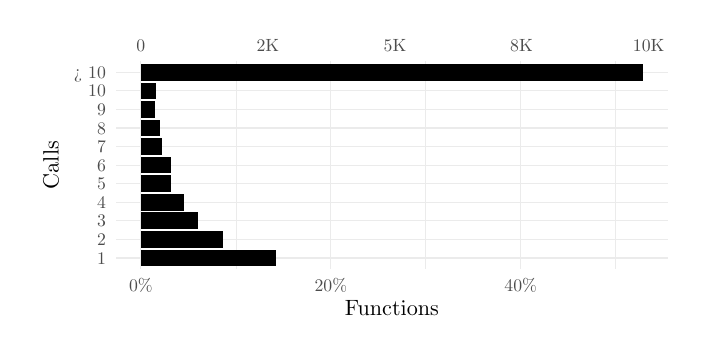
\begin{tikzpicture}[x=1pt,y=1pt]
\definecolor{fillColor}{RGB}{255,255,255}
\path[use as bounding box,fill=fillColor,fill opacity=0.00] (0,0) rectangle (238.49,108.41);
\begin{scope}
\path[clip] ( 31.86, 21.16) rectangle (231.38, 96.31);
\definecolor{drawColor}{gray}{0.92}

\path[draw=drawColor,line width= 0.2pt,line join=round] ( 75.23, 21.16) --
	( 75.23, 96.31);

\path[draw=drawColor,line width= 0.2pt,line join=round] (143.83, 21.16) --
	(143.83, 96.31);

\path[draw=drawColor,line width= 0.2pt,line join=round] (212.43, 21.16) --
	(212.43, 96.31);

\path[draw=drawColor,line width= 0.4pt,line join=round] ( 31.86, 25.19) --
	(231.38, 25.19);

\path[draw=drawColor,line width= 0.4pt,line join=round] ( 31.86, 31.90) --
	(231.38, 31.90);

\path[draw=drawColor,line width= 0.4pt,line join=round] ( 31.86, 38.61) --
	(231.38, 38.61);

\path[draw=drawColor,line width= 0.4pt,line join=round] ( 31.86, 45.32) --
	(231.38, 45.32);

\path[draw=drawColor,line width= 0.4pt,line join=round] ( 31.86, 52.03) --
	(231.38, 52.03);

\path[draw=drawColor,line width= 0.4pt,line join=round] ( 31.86, 58.73) --
	(231.38, 58.73);

\path[draw=drawColor,line width= 0.4pt,line join=round] ( 31.86, 65.44) --
	(231.38, 65.44);

\path[draw=drawColor,line width= 0.4pt,line join=round] ( 31.86, 72.15) --
	(231.38, 72.15);

\path[draw=drawColor,line width= 0.4pt,line join=round] ( 31.86, 78.86) --
	(231.38, 78.86);

\path[draw=drawColor,line width= 0.4pt,line join=round] ( 31.86, 85.57) --
	(231.38, 85.57);

\path[draw=drawColor,line width= 0.4pt,line join=round] ( 31.86, 92.28) --
	(231.38, 92.28);

\path[draw=drawColor,line width= 0.4pt,line join=round] ( 40.93, 21.16) --
	( 40.93, 96.31);

\path[draw=drawColor,line width= 0.4pt,line join=round] (109.53, 21.16) --
	(109.53, 96.31);

\path[draw=drawColor,line width= 0.4pt,line join=round] (178.13, 21.16) --
	(178.13, 96.31);
\definecolor{fillColor}{RGB}{0,0,0}

\path[fill=fillColor] ( 40.93, 89.26) rectangle (222.31, 95.30);

\path[fill=fillColor] ( 40.93, 22.17) rectangle ( 89.89, 28.21);

\path[fill=fillColor] ( 40.93, 28.88) rectangle ( 70.62, 34.92);

\path[fill=fillColor] ( 40.93, 35.59) rectangle ( 61.56, 41.63);

\path[fill=fillColor] ( 40.93, 42.30) rectangle ( 56.31, 48.34);

\path[fill=fillColor] ( 40.93, 55.72) rectangle ( 51.90, 61.75);

\path[fill=fillColor] ( 40.93, 49.01) rectangle ( 51.87, 55.04);

\path[fill=fillColor] ( 40.93, 62.43) rectangle ( 48.49, 68.46);

\path[fill=fillColor] ( 40.93, 69.13) rectangle ( 47.87, 75.17);

\path[fill=fillColor] ( 40.93, 82.55) rectangle ( 46.25, 88.59);

\path[fill=fillColor] ( 40.93, 75.84) rectangle ( 46.18, 81.88);
\end{scope}
\begin{scope}
\path[clip] (  0.00,  0.00) rectangle (238.49,108.41);
\definecolor{drawColor}{gray}{0.30}

\node[text=drawColor,anchor=base,inner sep=0pt, outer sep=0pt, scale=  0.64] at ( 40.85, 99.91) {0};

\node[text=drawColor,anchor=base,inner sep=0pt, outer sep=0pt, scale=  0.64] at ( 86.78, 99.91) {2K};

\node[text=drawColor,anchor=base,inner sep=0pt, outer sep=0pt, scale=  0.64] at (132.72, 99.91) {5K};

\node[text=drawColor,anchor=base,inner sep=0pt, outer sep=0pt, scale=  0.64] at (178.45, 99.91) {8K};

\node[text=drawColor,anchor=base,inner sep=0pt, outer sep=0pt, scale=  0.64] at (224.39, 99.91) {10K};
\end{scope}
\begin{scope}
\path[clip] (  0.00,  0.00) rectangle (238.49,108.41);
\definecolor{drawColor}{gray}{0.30}

\node[text=drawColor,anchor=base east,inner sep=0pt, outer sep=0pt, scale=  0.64] at ( 28.26, 22.98) {1};

\node[text=drawColor,anchor=base east,inner sep=0pt, outer sep=0pt, scale=  0.64] at ( 28.26, 29.69) {2};

\node[text=drawColor,anchor=base east,inner sep=0pt, outer sep=0pt, scale=  0.64] at ( 28.26, 36.40) {3};

\node[text=drawColor,anchor=base east,inner sep=0pt, outer sep=0pt, scale=  0.64] at ( 28.26, 43.11) {4};

\node[text=drawColor,anchor=base east,inner sep=0pt, outer sep=0pt, scale=  0.64] at ( 28.26, 49.82) {5};

\node[text=drawColor,anchor=base east,inner sep=0pt, outer sep=0pt, scale=  0.64] at ( 28.26, 56.53) {6};

\node[text=drawColor,anchor=base east,inner sep=0pt, outer sep=0pt, scale=  0.64] at ( 28.26, 63.24) {7};

\node[text=drawColor,anchor=base east,inner sep=0pt, outer sep=0pt, scale=  0.64] at ( 28.26, 69.95) {8};

\node[text=drawColor,anchor=base east,inner sep=0pt, outer sep=0pt, scale=  0.64] at ( 28.26, 76.66) {9};

\node[text=drawColor,anchor=base east,inner sep=0pt, outer sep=0pt, scale=  0.64] at ( 28.26, 83.37) {10};

\node[text=drawColor,anchor=base east,inner sep=0pt, outer sep=0pt, scale=  0.64] at ( 28.26, 90.08) {> 10};
\end{scope}
\begin{scope}
\path[clip] (  0.00,  0.00) rectangle (238.49,108.41);
\definecolor{drawColor}{gray}{0.30}

\node[text=drawColor,anchor=base,inner sep=0pt, outer sep=0pt, scale=  0.64] at ( 40.93, 13.15) {0{\%}};

\node[text=drawColor,anchor=base,inner sep=0pt, outer sep=0pt, scale=  0.64] at (109.53, 13.15) {20{\%}};

\node[text=drawColor,anchor=base,inner sep=0pt, outer sep=0pt, scale=  0.64] at (178.13, 13.15) {40{\%}};
\end{scope}
\begin{scope}
\path[clip] (  0.00,  0.00) rectangle (238.49,108.41);
\definecolor{drawColor}{RGB}{0,0,0}

\node[text=drawColor,anchor=base,inner sep=0pt, outer sep=0pt, scale=  0.80] at (131.62,  4.40) {Functions};
\end{scope}
\begin{scope}
\path[clip] (  0.00,  0.00) rectangle (238.49,108.41);
\definecolor{drawColor}{RGB}{0,0,0}

\node[text=drawColor,rotate= 90.00,anchor=base,inner sep=0pt, outer sep=0pt, scale=  0.80] at ( 11.20, 58.73) {Calls};
\end{scope}
\end{tikzpicture}

  \caption{Call Distribution}
  \label{fig:calldist}
\end{figure}

These functions have a total of 67,225 parameter positions.
Figure~\ref{fig:paramdist} shows the distribution of parameter positions.
3.0\% functions have 0 parameters, 22.4\% have 1, and 5.0\% have over
10. There are 4 functions with over 50 parameters that come from 3 packages. Of
those, \texttt{ggplot2::theme} has the highest, 95 parameters.

\begin{figure}[!h]
  \centering
  % Created by tikzDevice version 0.12.3.1 on 2021-06-03 17:14:19
% !TEX encoding = UTF-8 Unicode
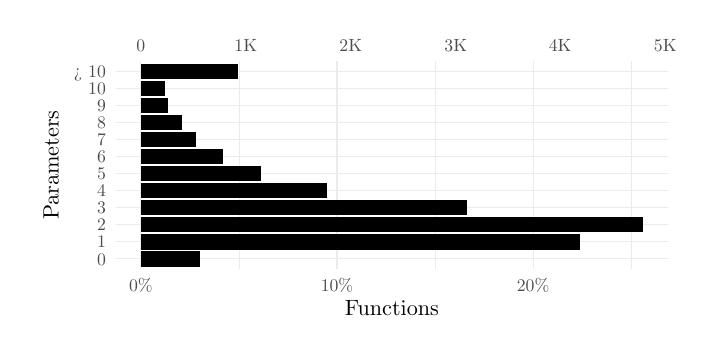
\begin{tikzpicture}[x=1pt,y=1pt]
\definecolor{fillColor}{RGB}{255,255,255}
\path[use as bounding box,fill=fillColor,fill opacity=0.00] (0,0) rectangle (238.49,108.41);
\begin{scope}
\path[clip] ( 31.86, 21.16) rectangle (231.38, 96.31);
\definecolor{drawColor}{gray}{0.92}

\path[draw=drawColor,line width= 0.2pt,line join=round] ( 76.35, 21.16) --
	( 76.35, 96.31);

\path[draw=drawColor,line width= 0.2pt,line join=round] (147.19, 21.16) --
	(147.19, 96.31);

\path[draw=drawColor,line width= 0.2pt,line join=round] (218.04, 21.16) --
	(218.04, 96.31);

\path[draw=drawColor,line width= 0.4pt,line join=round] ( 31.86, 24.86) --
	(231.38, 24.86);

\path[draw=drawColor,line width= 0.4pt,line join=round] ( 31.86, 31.02) --
	(231.38, 31.02);

\path[draw=drawColor,line width= 0.4pt,line join=round] ( 31.86, 37.18) --
	(231.38, 37.18);

\path[draw=drawColor,line width= 0.4pt,line join=round] ( 31.86, 43.34) --
	(231.38, 43.34);

\path[draw=drawColor,line width= 0.4pt,line join=round] ( 31.86, 49.50) --
	(231.38, 49.50);

\path[draw=drawColor,line width= 0.4pt,line join=round] ( 31.86, 55.66) --
	(231.38, 55.66);

\path[draw=drawColor,line width= 0.4pt,line join=round] ( 31.86, 61.81) --
	(231.38, 61.81);

\path[draw=drawColor,line width= 0.4pt,line join=round] ( 31.86, 67.97) --
	(231.38, 67.97);

\path[draw=drawColor,line width= 0.4pt,line join=round] ( 31.86, 74.13) --
	(231.38, 74.13);

\path[draw=drawColor,line width= 0.4pt,line join=round] ( 31.86, 80.29) --
	(231.38, 80.29);

\path[draw=drawColor,line width= 0.4pt,line join=round] ( 31.86, 86.45) --
	(231.38, 86.45);

\path[draw=drawColor,line width= 0.4pt,line join=round] ( 31.86, 92.61) --
	(231.38, 92.61);

\path[draw=drawColor,line width= 0.4pt,line join=round] ( 40.93, 21.16) --
	( 40.93, 96.31);

\path[draw=drawColor,line width= 0.4pt,line join=round] (111.77, 21.16) --
	(111.77, 96.31);

\path[draw=drawColor,line width= 0.4pt,line join=round] (182.62, 21.16) --
	(182.62, 96.31);
\definecolor{fillColor}{RGB}{0,0,0}

\path[fill=fillColor] ( 40.93, 89.84) rectangle ( 76.18, 95.38);

\path[fill=fillColor] ( 40.93, 22.09) rectangle ( 62.34, 27.63);

\path[fill=fillColor] ( 40.93, 28.25) rectangle (199.57, 33.79);

\path[fill=fillColor] ( 40.93, 83.68) rectangle ( 49.80, 89.22);

\path[fill=fillColor] ( 40.93, 34.41) rectangle (222.31, 39.95);

\path[fill=fillColor] ( 40.93, 40.56) rectangle (158.76, 46.11);

\path[fill=fillColor] ( 40.93, 46.72) rectangle (108.20, 52.27);

\path[fill=fillColor] ( 40.93, 52.88) rectangle ( 84.25, 58.43);

\path[fill=fillColor] ( 40.93, 59.04) rectangle ( 70.64, 64.59);

\path[fill=fillColor] ( 40.93, 65.20) rectangle ( 60.94, 70.75);

\path[fill=fillColor] ( 40.93, 71.36) rectangle ( 55.94, 76.91);

\path[fill=fillColor] ( 40.93, 77.52) rectangle ( 50.67, 83.06);
\end{scope}
\begin{scope}
\path[clip] (  0.00,  0.00) rectangle (238.49,108.41);
\definecolor{drawColor}{gray}{0.30}

\node[text=drawColor,anchor=base,inner sep=0pt, outer sep=0pt, scale=  0.64] at ( 40.85, 99.91) {0};

\node[text=drawColor,anchor=base,inner sep=0pt, outer sep=0pt, scale=  0.64] at ( 78.80, 99.91) {1K};

\node[text=drawColor,anchor=base,inner sep=0pt, outer sep=0pt, scale=  0.64] at (116.74, 99.91) {2K};

\node[text=drawColor,anchor=base,inner sep=0pt, outer sep=0pt, scale=  0.64] at (154.69, 99.91) {3K};

\node[text=drawColor,anchor=base,inner sep=0pt, outer sep=0pt, scale=  0.64] at (192.43, 99.91) {4K};

\node[text=drawColor,anchor=base,inner sep=0pt, outer sep=0pt, scale=  0.64] at (230.38, 99.91) {5K};
\end{scope}
\begin{scope}
\path[clip] (  0.00,  0.00) rectangle (238.49,108.41);
\definecolor{drawColor}{gray}{0.30}

\node[text=drawColor,anchor=base east,inner sep=0pt, outer sep=0pt, scale=  0.64] at ( 28.26, 22.65) {0};

\node[text=drawColor,anchor=base east,inner sep=0pt, outer sep=0pt, scale=  0.64] at ( 28.26, 28.81) {1};

\node[text=drawColor,anchor=base east,inner sep=0pt, outer sep=0pt, scale=  0.64] at ( 28.26, 34.97) {2};

\node[text=drawColor,anchor=base east,inner sep=0pt, outer sep=0pt, scale=  0.64] at ( 28.26, 41.13) {3};

\node[text=drawColor,anchor=base east,inner sep=0pt, outer sep=0pt, scale=  0.64] at ( 28.26, 47.29) {4};

\node[text=drawColor,anchor=base east,inner sep=0pt, outer sep=0pt, scale=  0.64] at ( 28.26, 53.45) {5};

\node[text=drawColor,anchor=base east,inner sep=0pt, outer sep=0pt, scale=  0.64] at ( 28.26, 59.61) {6};

\node[text=drawColor,anchor=base east,inner sep=0pt, outer sep=0pt, scale=  0.64] at ( 28.26, 65.77) {7};

\node[text=drawColor,anchor=base east,inner sep=0pt, outer sep=0pt, scale=  0.64] at ( 28.26, 71.93) {8};

\node[text=drawColor,anchor=base east,inner sep=0pt, outer sep=0pt, scale=  0.64] at ( 28.26, 78.09) {9};

\node[text=drawColor,anchor=base east,inner sep=0pt, outer sep=0pt, scale=  0.64] at ( 28.26, 84.25) {10};

\node[text=drawColor,anchor=base east,inner sep=0pt, outer sep=0pt, scale=  0.64] at ( 28.26, 90.41) {> 10};
\end{scope}
\begin{scope}
\path[clip] (  0.00,  0.00) rectangle (238.49,108.41);
\definecolor{drawColor}{gray}{0.30}

\node[text=drawColor,anchor=base,inner sep=0pt, outer sep=0pt, scale=  0.64] at ( 40.93, 13.15) {0{\%}};

\node[text=drawColor,anchor=base,inner sep=0pt, outer sep=0pt, scale=  0.64] at (111.77, 13.15) {10{\%}};

\node[text=drawColor,anchor=base,inner sep=0pt, outer sep=0pt, scale=  0.64] at (182.62, 13.15) {20{\%}};
\end{scope}
\begin{scope}
\path[clip] (  0.00,  0.00) rectangle (238.49,108.41);
\definecolor{drawColor}{RGB}{0,0,0}

\node[text=drawColor,anchor=base,inner sep=0pt, outer sep=0pt, scale=  0.80] at (131.62,  4.40) {Functions};
\end{scope}
\begin{scope}
\path[clip] (  0.00,  0.00) rectangle (238.49,108.41);
\definecolor{drawColor}{RGB}{0,0,0}

\node[text=drawColor,rotate= 90.00,anchor=base,inner sep=0pt, outer sep=0pt, scale=  0.80] at ( 11.20, 58.73) {Parameters};
\end{scope}
\end{tikzpicture}

  \caption{Parameter Distribution}
  \label{fig:paramdist}
\end{figure}

\section{Analyzing Environment Usage Patterns}

\subsection{Life Cycle of Environments}
In our corpus, we observe the creation of 1.2 B environments, which makes them
the second most widely allocated objects. Table~\ref{table:object_count_dist}
shows the distribution of R objects for comparison. Promises are the most widely
allocated objects, studied extensively by \citet{oopsla19b}. Vectors of logicals
and characters (string) are more frequently allocated compared to that of
integers, reals, and raw (bytes). Language objects, i.e, first-class
expressions, are used for metaprogramming. Lists are heterogeneous vectors.
Other objects such as S4, externalptr, etc. are rare.

\begin{table}
  \vspace{-3mm}
  \small
  \caption{Object Counts} \label{table:object_count_dist}
  \centering
  \begin{tabular}{lr}
    \toprule
    \textbf{Type}&\textbf{Count}\\
    \midrule
    Promise&3.0B\\
    Environment&1.2B\\
    Logical&1.1B\\
    Character&976.9M\\
    Language&506.6M\\
    Integer&482.0M\\
    \bottomrule
  \end{tabular}
  \begin{tabular}{lr}
    \toprule
    \textbf{Type}&\textbf{Count}\\
    \midrule
    List&168.2M\\
    Real&127.2M\\
    Closure&118.5M\\
    Symbol&74.3M\\
    Raw&50.1M\\
    Other&15.9M\\
    \bottomrule
  \end{tabular}
\end{table}

\paragraph{Where do environments come from?} The distribution of environments by
source is presented in Table~\ref{table:env_source}. The columns of this table
are to be read as follows. \emph{Core} represents the GNU R implementation and
its 16 packages: \code{base}, \code{compiler}, \code{datasets},
\code{grDevices}, \code{graphics}, \code{grid}, \code{methods}, \code{parallel},
\code{profile}, \code{splines}, \code{stats}, \code{stats4}, \code{tcltk},
\code{tools}, \code{translations}, and \code{utils}. \emph{User} represents CRAN
packages. \emph{Native} represents environment creation using the C APIs
\code{allocSExp}, \code{Rf_NewEnvironment}, and \code{Rf_NewHashedEnv}. Only
\code{allocSexp} is exported for use by external packages. \emph{R} represents
environment creation using \newEnv. \emph{Foreign} represents environments that
were created outside of the code being traced; hence they are ignored from the
rest of the discussion.

The R core is responsible for 99.89\% of the environments, dominated by
\emph{Native} . User packages are responsible for 0.03\% of the environments,
with twice as many from \emph{R} as \emph{Native}.

\begin{table}[!h]
  \vspace{-3mm}
  \small
  \centering
  \caption{Environment Source}\label{table:env_source}
  \vspace{-3mm}
  \begin{tabular}{llrr}
    \toprule
    \multirow{2}{*}{Core}  & \multicolumn{1}{l}{Native} & \multicolumn{1}{r}{1.1B} & \multicolumn{1}{r}{99.62\%}\\
                           & \multicolumn{1}{l}{R}     & \multicolumn{1}{r}{3.1M} & \multicolumn{1}{r}{0.27\%}\\
    \midrule
    \multirow{2}{*}{User}  & \multicolumn{1}{l}{Native} & \multicolumn{1}{r}{163.6K} & \multicolumn{1}{r}{0.01\%}\\
                           & \multicolumn{1}{l}{R}      & \multicolumn{1}{r}{239.3K} & \multicolumn{1}{r}{0.02\%}\\
    \midrule
    Foreign & &\multicolumn{1}{r}{899.6K} & \multicolumn{1}{r}{0.08\%}\\
    \bottomrule
  \end{tabular}
\end{table}


\emph{Core}, \emph{Native} environments: 99.7\% of environments in this category
are used for function calls, 334.5K are package namespaces, 2.9M are created by
the \code{methods} package for S4 object-oriented system, and 175K by the
\code{base} package for dynamic evaluation using \code{eval} and for registering
native functions from R packages for access by other R packages.

\emph{Core}, \emph{R} environments: 94.1\% of these environments are created by
\code{base}, and 5.3\% by \code{methods} for the S4 object-oriented system. The
\code{base} package contribution comes from an internal function,
\code{lazyLoadDBexec}, used for loading package code and processed help files
from binary files.

\emph{User} environments: These environments come from many packages and are
used for a variety of purposes such as hash tables, objects for custom OOP
systems, sandboxing, etc.

\begin{table}
  \vspace{-3mm}
  \small
  \caption{Environment Source} \label{table:env_source_dist}
  \centering
  \begin{tabular}{l|rr}
    \toprule
    \textbf{Source}&\textbf{Count}&\textbf{Percentage}\\
    \midrule
    Call&1.2B&99.4\%\\
    Other&7.2M&0.6\%\\
    Package&672.5K&0.1\%\\
    \bottomrule
  \end{tabular}
\end{table}


\paragraph{What are environment life-cycles?} To characterize the life-cycle of
environments, we summarize the sequence of events that affect it. The events of
interest are \underline{S}ubstitute, \underline{P}arent.frame,
s\underline{Y}s.frame, \underline{G}et, \underline{E}nvironment,
\underline{A}rgument for environments passed as arguments to other functions and
\underline{R}eturn for environments returned from functions. Events occurring to
an environment passed to \eval are enclosed by $[$ and $]$. The event sequence
of a call environment after the call has ended is preceded by a $\#$.


\section{Explicit Environment Creation}
In this section, we discuss explicit environment creation using the \newEnv R
function. We observe 3.3M environments created using this function. The GNU R
implementation (\base package) accounts for 87\% (2.9M) of these and packages
contribute remaining 13\% (420.6K).

The implementation environments all come from a single \base package function,
\lazyLoadDBexec, used only internally. This function is responsible for loading
a package's code from a binary file and also for loading processed help file
data. Since this is an implementation detail, we ignore this for the rest of the
discussion.

There are 59 packages responsible for all the remaining calls to \newEnv.
Table~\ref{table:pack_env} shows the distribution of \newEnv calls for the top
14 packages.

\begin{table}[!h]
  \vspace{-3mm}
  \small
  \caption{Package Explicit Environments} \label{table:pack_env}
  \centering
  \begin{tabular}{lrr}
    \toprule
    \textbf{Package}&\textbf{\#}&\textbf{Cum. \%}\\
    \midrule
    methods&161.6K&38.4\%\\
    rlang&75.0K&56.3\%\\
    R6&73.8K&73.8\%\\
    codetools&38.9K&83.1\%\\
    ggplot2&24.3K&88.8\%\\
    grid&15.7K&92.6\%\\
    testthat&9.0K&94.7\%\\
    \bottomrule
  \end{tabular}
  \begin{tabular}{lrr}
    \toprule
    \textbf{Package}&\textbf{\#}&\textbf{Cum. \%}\\
    \midrule
    dplyr&8.2K&96.7\%\\
    stats&2.7K&97.3\%\\
    forecast&1.5K&97.7\%\\
    data.table&1.5K&98.0\%\\
    plyr&1.2K&98.3\%\\
    ps&1.1K&98.5\%\\
    cli&846.0&98.7\%\\
    \bottomrule
  \end{tabular}
\end{table}

The \methods package alone is responsible for 38.4\% of these calls. This
package ships with GNU R and implements the S4 object-oriented system, a
multi-argument dynamic dispatch system. The top 6 packages account for 92.6\% of
the calls.

\subsection{Explicit Environments}

\subsubsection{User Explicit Environments}

\begin{table}[!h]
  \vspace{-3mm}
  \small
  \caption{User Explicit Environment Sequence} \label{table:user_explicit_env_seq}
  \centering
  \begin{tabular}{lrr}
    \toprule
    \textbf{Event Sequence}&\textbf{\#}&\textbf{Cum. \%}\\
    \midrule
    \texttt{A*}&151.9K&38.8\%\\
    \texttt{N A*}&97.6K&63.7\%\\
    \texttt{N A* !+}&43.7K&74.8\%\\
    \texttt{N !* A* L+ !* @?}&41.4K&85.4\%\\
    \texttt{N A* @ A*}&38.8K&95.3\%\\
    \texttt{N [ A* ]}&3.8K&96.3\%\\
    \texttt{N !* @ !*}&3.1K&97.1\%\\
    \bottomrule
  \end{tabular}
\end{table}

The first sequence, \texttt{N A*}, represents 63.7\% of the environments. These
environments are created and variables are added, looked up or removed from
them. These environments come from 35 packages. They are used for a variety of
purposes; storing package and custom object state being the most common use. The
next sequence \texttt{N A* !+} involves inheritance of the environment by a
another environment, either by passing it as the \code{parent} argument to
\code{new.env} or explicitly setting it as a parent using \code{parent.env<-}.
This sequence originates from packages like R6 and R.oo which implement OO
systems and rlang which implements an alternate API for R including one for
creating new environments. This is following by the sequence \texttt{N !* A* L+
  !* @?}, coming exclusively from \code{R6}. It features two new events:
\texttt{L} locks the environment and its bindings to protect from further
modifications, and \texttt{@} sets attributes on the environment. This sequence
is a signature for the \code{R6} package which implements an object oriented
system. The next sequence, \texttt{N A* @ A*}, represents the creation of
environment, and setting an attribute. An example is the \code{XML} package
which creates a \code{hashTree} object and sets the attribute
\code{XMLHashTree}. After this, we have environments that are created for the
purpose of evaluating code, explained by the sequence \texttt{N [ A* ]}. This is
a common pattern in many packages implementing custom evaluation strategies,
such as glue testthat, shiny, and rlang. Finally, the last sequence involves
environments that are created, inherited and an attribute is set on them. An
example of this pattern is the indexing semantics of immutable data frames
created by the \code{plyr} package. It creates a new environment and sets it as
a parent of functions to customize the treatment of the indexed data frame.

The most common user of explicit environments is
\code{vec_c} function. via

The \code{foreach} package provides a looping construct to execute R code,
optionally in parallel. It creates an iterator for sequences of values. The
dynamic state of the iterator, updated on each iteration, is represented using
an explicit environment extending the empty environment. The 

\begin{table}[!h]
  \vspace{-3mm}
  \small
  \caption{Core Explicit Environment Sequence} \label{table:core_explicit_env_seq}
  \centering
  \begin{tabular}{lrr}
    \toprule
    \textbf{Event Sequence}&\textbf{\#}&\textbf{Cum. \%}\\
    \midrule
    \texttt{A*}&2.9M&90.8\%\\
    \texttt{S}&144.8K&95.4\%\\
    \texttt{[ A* ]}&140.7K&99.9\%\\
    \bottomrule
  \end{tabular}
\end{table}

\bibliography{bib/jv,bib/aviral}



\end{document}

% TODO
% - environment source
%            C   new.env
% - base
% - library
%
% environment class
% - 
